\documentclass[11pt]{article}

\usepackage{kotex}
\usepackage{graphicx}
\usepackage{amsmath}
\usepackage{tikz}

\graphicspath{{../images/}}

\begin{document}
Hello world!

\begin{figure}[t]
\centering\includegraphics[scale=0.5]{eps.png}
\caption{\texttt{\symbol{92}includegraphics} 명령으로 부른 그림(축소/확대) \label{fig:texgr01}}
\end{figure}

\begin{figure}[t]
\centering\includegraphics[width=0.97\textwidth, height=5cm]{../images/eps.png}
\caption{\texttt{\symbol{92}includegraphics} 명령으로 부른 그림(축소/확대) \label{fig:texgr02}}
\end{figure}

\begin{figure}[t]
\caption{\texttt{\symbol{92}includegraphics}로 그림 일부만 잘로오기 \label{fig:texgr03}}
\centering\includegraphics*[300pt, 0pt][600pt, 150pt]{eps.png}
\end{figure}

\begin{figure}[t]
\caption{\texttt{\symbol{92}includegraphics}로 그림 일부만 잘로오기 \label{fig:texgr04}}
\centering\includegraphics*[bb=300 0 600 150, width=0.5\textwidth, height=.4\textwidth]{eps.png}
\end{figure}

\begin{figure}[t]
\begin{center}
\includegraphics[width=1.8in]{play.png}
\includegraphics[width=1.8in, angle=-30]{play.png}
\caption[그림의 회전]{PostScript 그림 \texttt{play.png}의 원본 및 반시계 방향으로 30\textdegree 회전한 결과 \label{fig:play}}
\end{center}
\end{figure}

\begin{figure}[t]
왼쪽 문자--
\includegraphics*[bb=14 64 70 85]{eps.png}
--오른쪽 문자
\caption{\texttt{*} 있는 \texttt{\symbol{92}includegraphics*}명령 \label{fig:include*}}
\end{figure}

\begin{figure}[t]
왼쪽 문자--
\includegraphics*[bb=14 64 70 85]{eps.png}
--오른쪽 문자
\caption{\texttt{*} 없는 \texttt{\symbol{92}includegraphics 명령 \label{fig:include0}}}
\end{figure}

\begin{figure}[t]
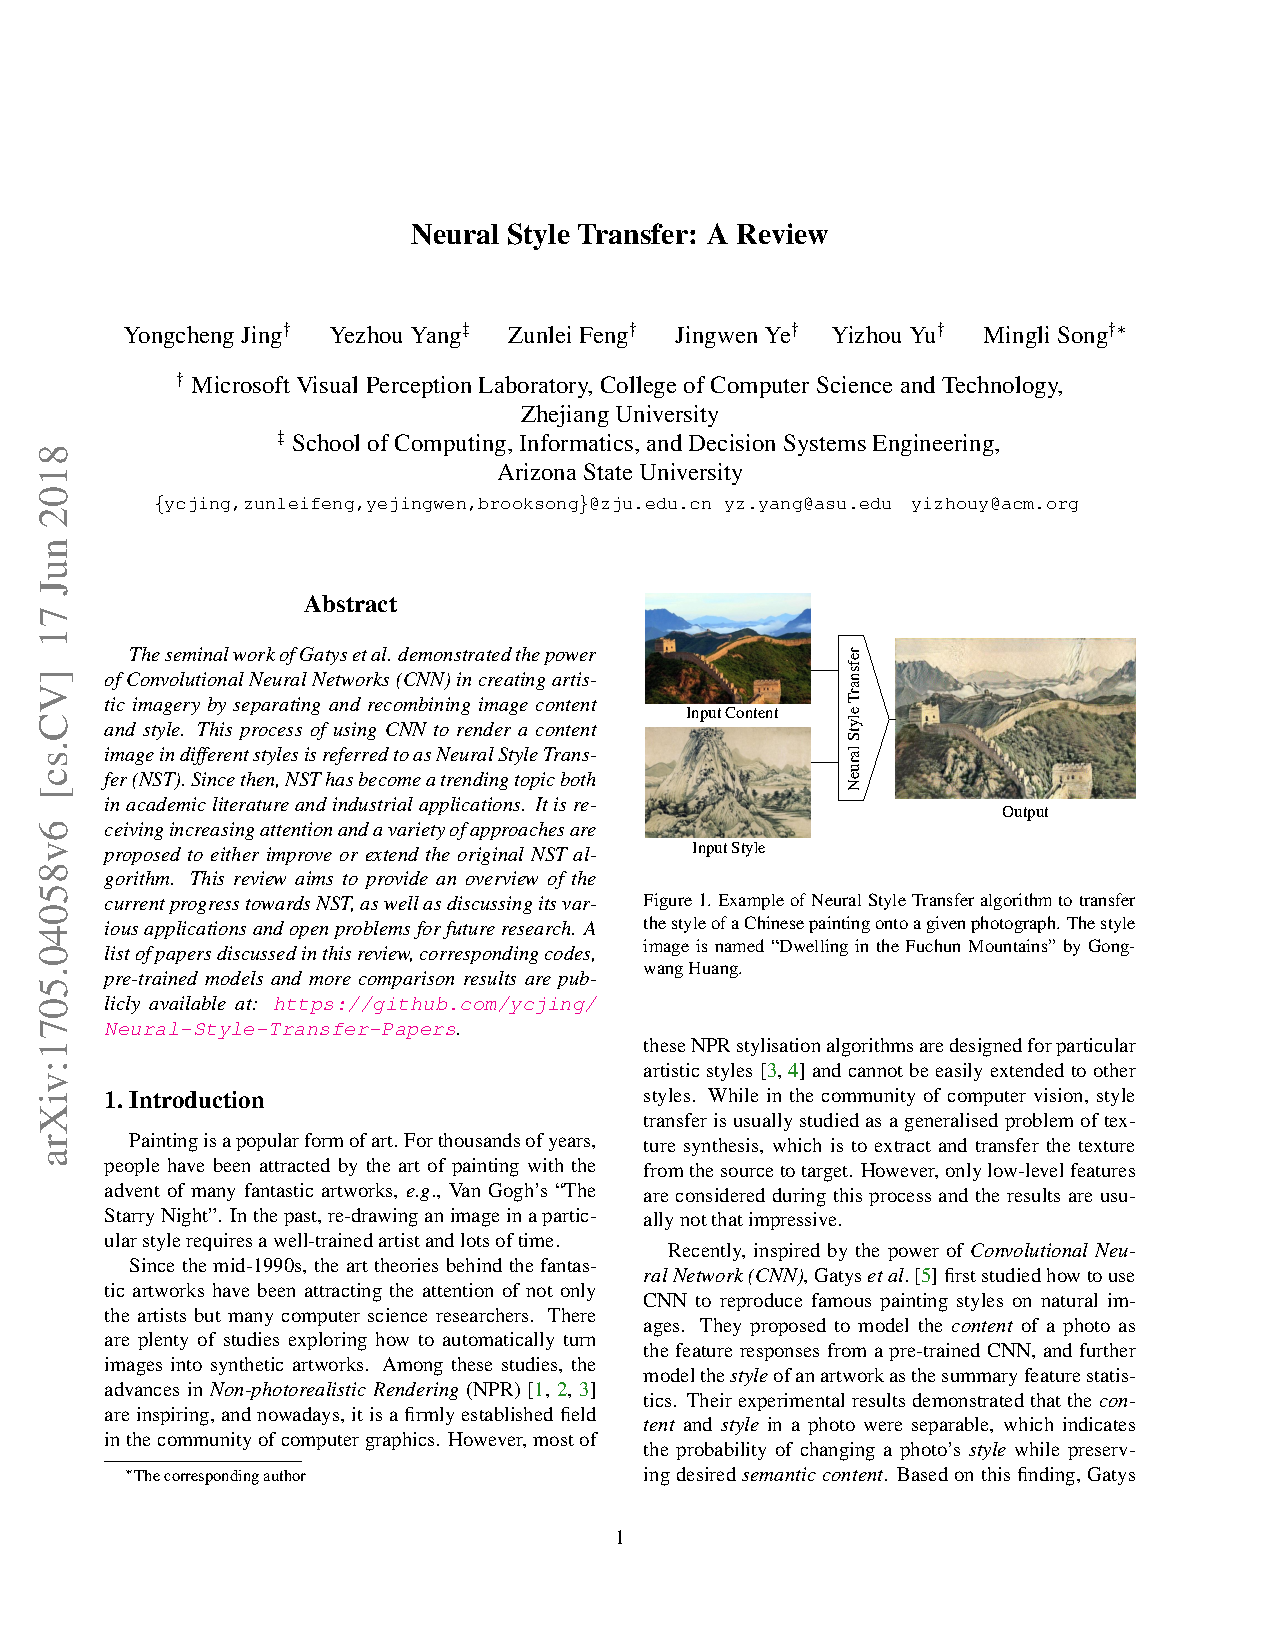
\includegraphics[width=0.5\textwidth, page=1]{style.pdf}
\caption{read pdf file}
\end{figure}

\begin{figure}[!t]
\noindent
\begin{minipage}[t]{2.5in}
\centerline{\includegraphics[scale=0.5]{play.png}}
\centerline{(a) 왼쪽 그림}
\end{minipage}
\begin{minipage}[t]{2.5in}
\centerline{\includegraphics[scale=0.5]{play.png}}
\centerline{(b) 오른쪽 그림}
\end{minipage}
\caption{왼쪽과 오른쪽 그림 \label{fig:combi}}
\end{figure}

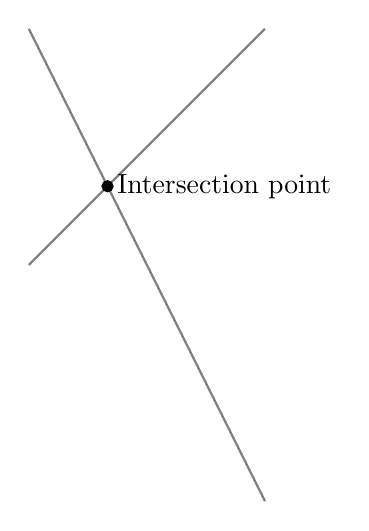
\begin{tikzpicture}
\draw[gray, thick] (-1,2) -- (2,-4);
\draw[gray, thick] (-1,-1) -- (2,2);
\filldraw[black] (0,0) circle (2pt) node[anchor=west] {Intersection point};
\end{tikzpicture}

\begin{minipage}[c]{2.1in}
오른쪽 그림과 같이, 함수 $f(x)=x^3-x^2$의 그래프 위의 점 $(a_0, f(a_0))$에서 접선을 긋고 (단 $a_0>3$) $x$축과의 교점을 $(a_1,0)$이라 한다. 다음에 점 $(a_1, f(a_1))$에서 접선을 긋고 $x$축과의 교점을 $(a_2,0)$ 이라 한다. 이러한 방법으로 계속하여 일반적으로 점 $(a_{n-1},f(a_{n-1}))$에서 접선을 긋고 $x$축과의 교점을 $(a_n,0)$이라 한다. 이때 다음 물음에 답하여라.
\end{minipage}
\ \hfill \
%\begin{minipage}{2.4in}
%\begin{tikzpicture}[xscale=2.25, yscale=2.5]
%\draw[thick,->](-0.7,0) -- (1.8,0) node[right] at (1.8,0) {$x$}; % x 축
%\draw[thick,->](0,-0.5) -- (0,1.5) node[below left] at (0,1.5) {$y$}; % y축
%\draw[black, domain=-0.5:1.6] plot (\x, {\x*\x*(\x-1)});
%\draw(1.05, 0) -- (1.2, 0.288) node[below] at (1.05, 0){\small$a_2$};
%\draw[dotted] (1.2, 0.288) -- (1.2,0);
%\draw (1.2,0) -- (1.5,1.125) node[right=2mm,below] at (1.2,0) %{\small$a_1$}
%\draw[dotted] (1.5, 1.125) -- (1.5, 0) node[below] at (1.5,0) {\small$a_0$};
%\end{tikzpicture}
%\end{minipage}
\begin{enumerate}
\item $a_n$을 $a_{n-1}$의 식으로 나타내어라 $(n=1,2,\cdots)$.
\item $a_0>a_1>a_2>\cdots>a_n>\cdots \geq \sqrt{3}$이 됨을 보여라.
\item $\displaystyle{\lim_{n \rightarrow \infty}}a_n$을 구하여라.
\end{enumerate}

\end{document}